\documentclass[a4paper]{ctexart}
\usepackage[section]{placeins}
\usepackage{enumerate}
\usepackage[top=1in, bottom=1in, left=1.25in, right=1.25in]{geometry}
\usepackage{graphicx}
\usepackage{listings}

\author{\\\\\\\\\\\\\\\\REMOVED<REMOVED>\\学号:REMOVED\\班级: REMOVED\\REMOVED\\\\\\\\\\\\\\}
\title{微机原理实验4\\STM32的USART串口功能实践}
\begin{document}

\begin{titlepage}
\maketitle
\thispagestyle{empty}
\newpage
\tableofcontents
\thispagestyle{empty}
\end{titlepage}

\setcounter{page}{1}
\lstset{language=C, 
    numbers=left, 
    frame=single,
    breaklines=true,
    breakautoindent=false,
    numberstyle=\tiny,
    fontadjust,
    basicstyle=\ttfamily
    }

\section{题目简介} 

使用STM32内置的USART串口功能,借助PC机上的通信工具,与上位机进行通信。

\section{题目分析}

由于串口通信设备没有回环功能,因此这里我要用STM32实现串口通信的回环,即把输入内容原封
不动的展示在屏幕上。“原封不动”在技术上比较难定义,因此这里我们只要实现:在picocom软件
中,以设定好的波特率通信时,可将发送的中、英文文字完整的返回,并正确的响应退格键和回车
键。

这个题目涉及到的技术细节有:
\begin{enumerate}[1.]
\item GPIO端口以及时钟配置
\item 片上的串口通信设备
\item 简单程序开发技巧
\end{enumerate}
下面对这几个要点分别进行说明

\subsection{GPIO端口以及时钟配置}

串口通信是由Rx、Tx两根线实现数据传输,并用GND线作为电平基准的一种差分通信方式。因此,
对于Rx和Tx两根线,也应该用不同的方式配置。根据下图\ref{stm32iodriver}的端口驱动电路,
以及图\ref{iso7816usartspecific}中所规定的LIN电平标准,应该使用浮空输入方式作为输入(
Rx)管脚的接入方式,而使用推挽输出或其他强输出方式作为输出管脚(Tx)的接入方式。
\begin{figure}[h]
  \centering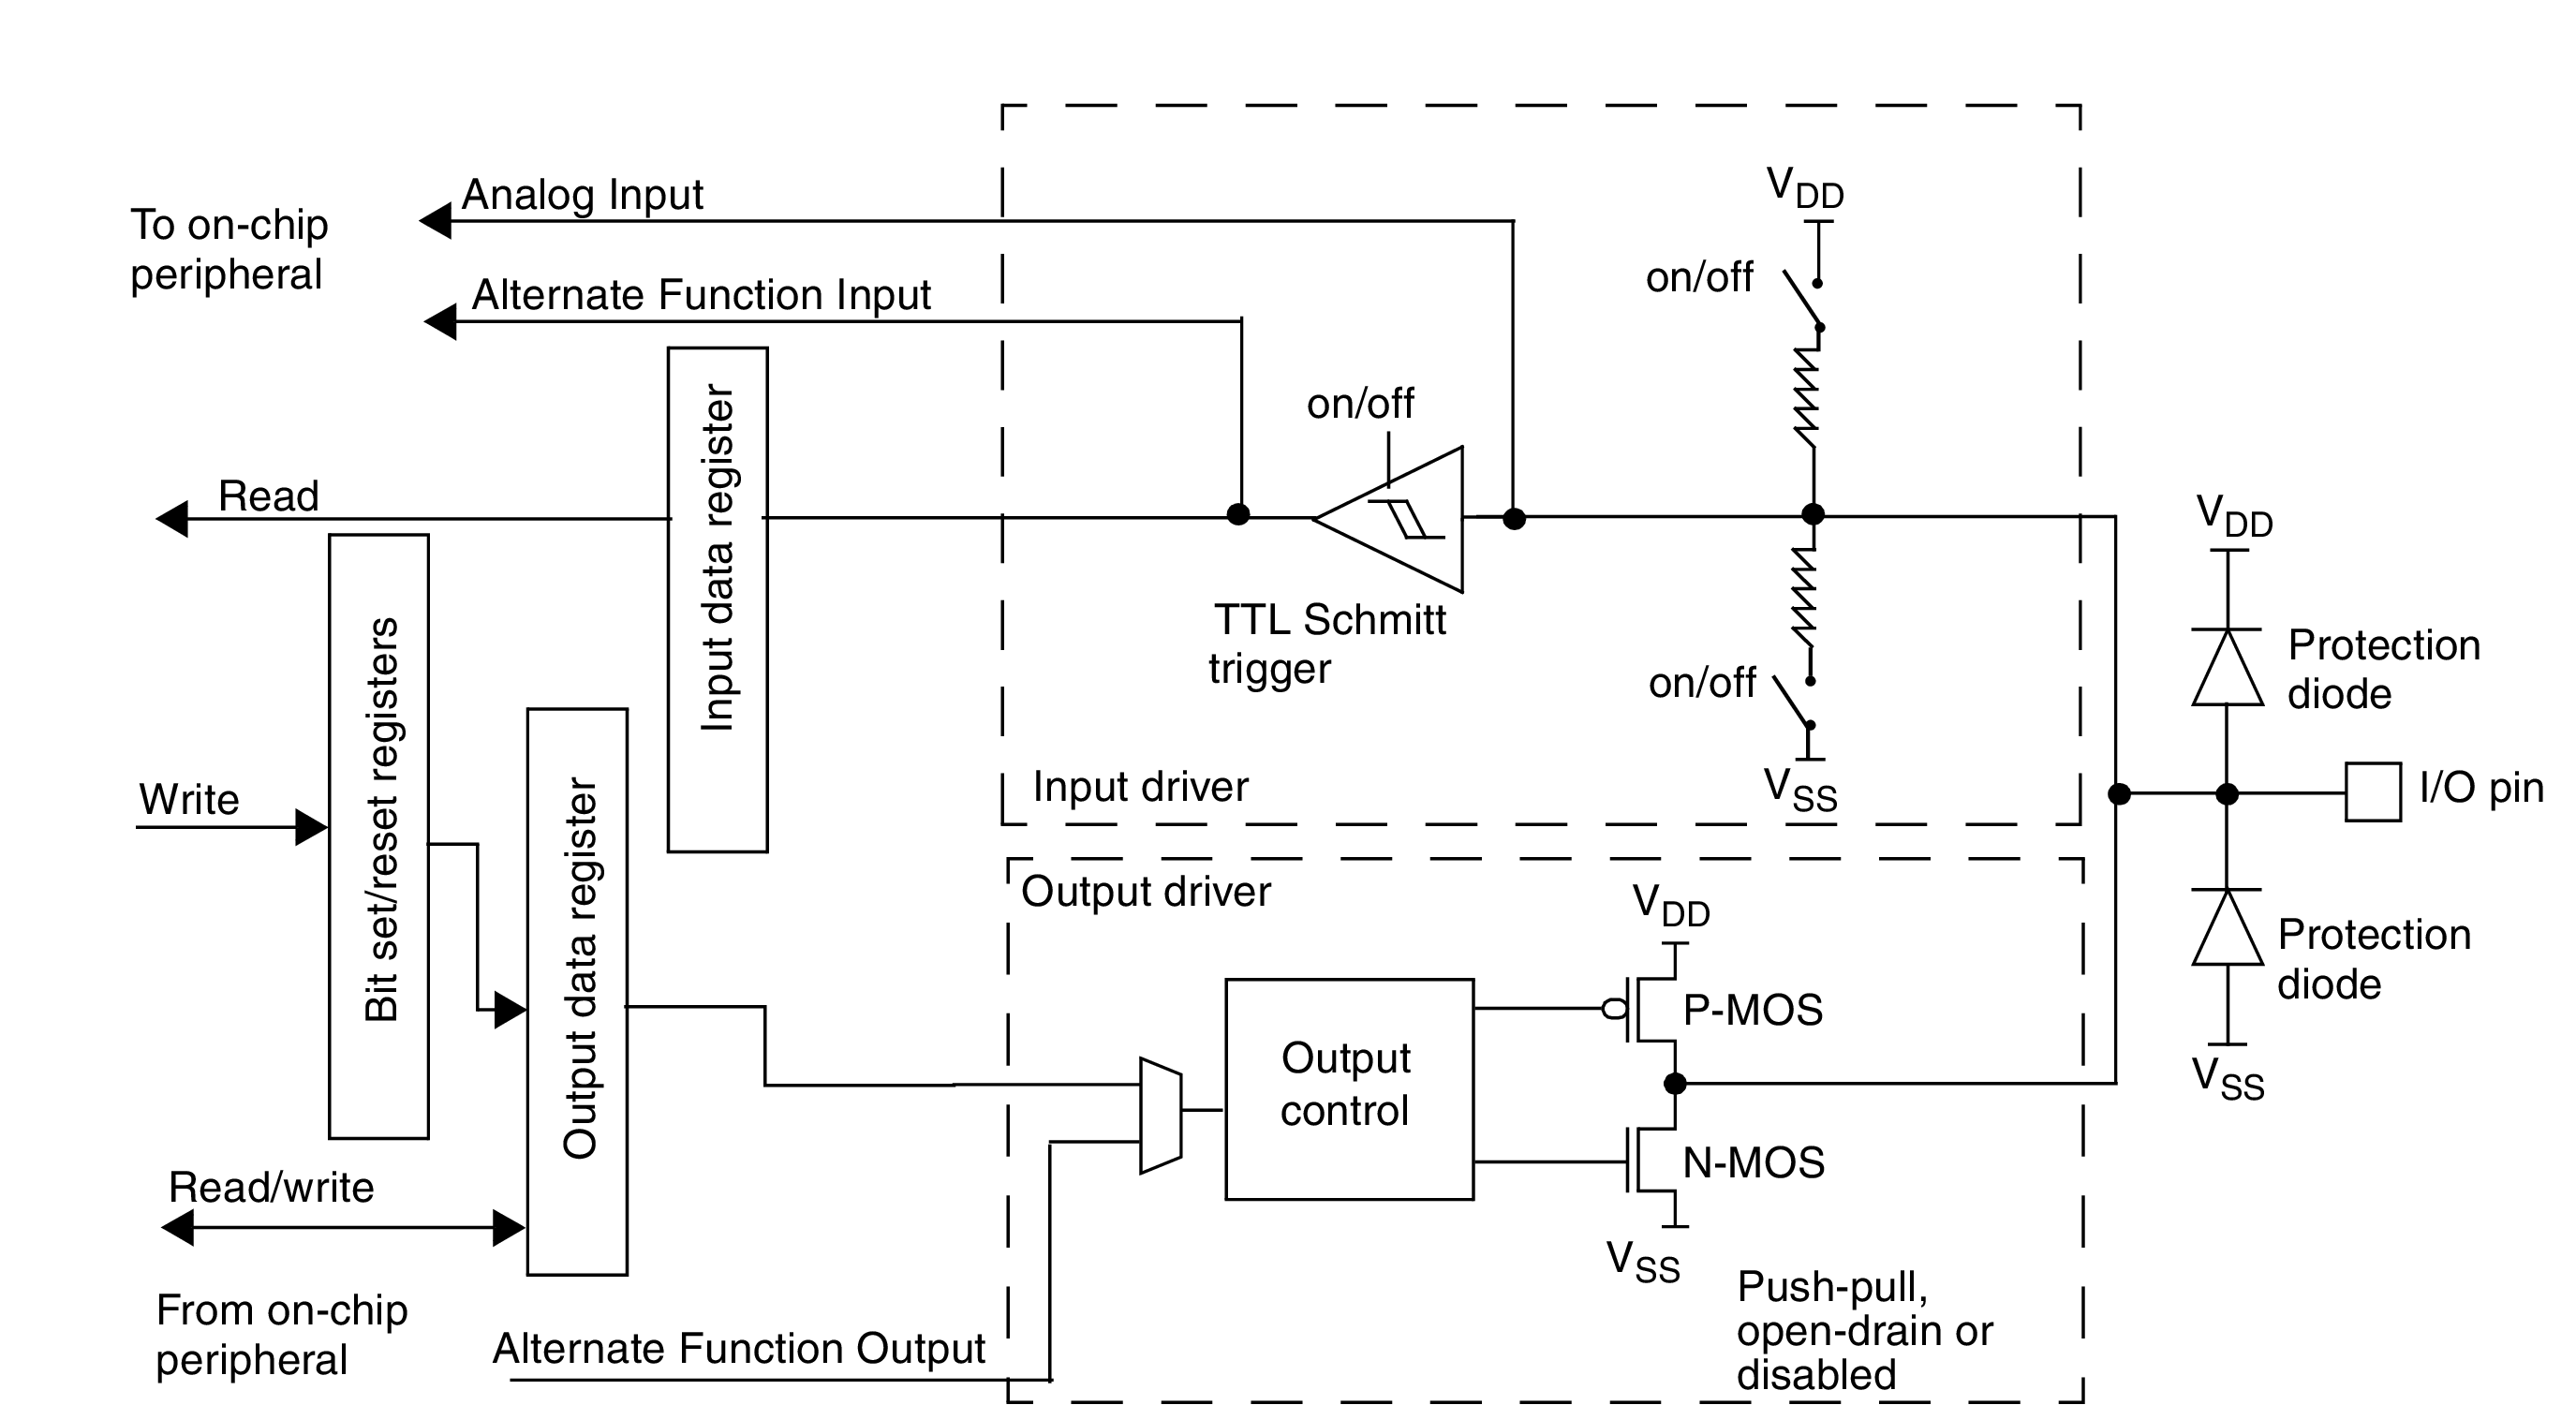
\includegraphics[width=\textwidth]{./img/ioport.png}
  \caption{STM32 IO Driver System}\label{stm32iodriver}
\end{figure}
\begin{figure}[h]
  \centering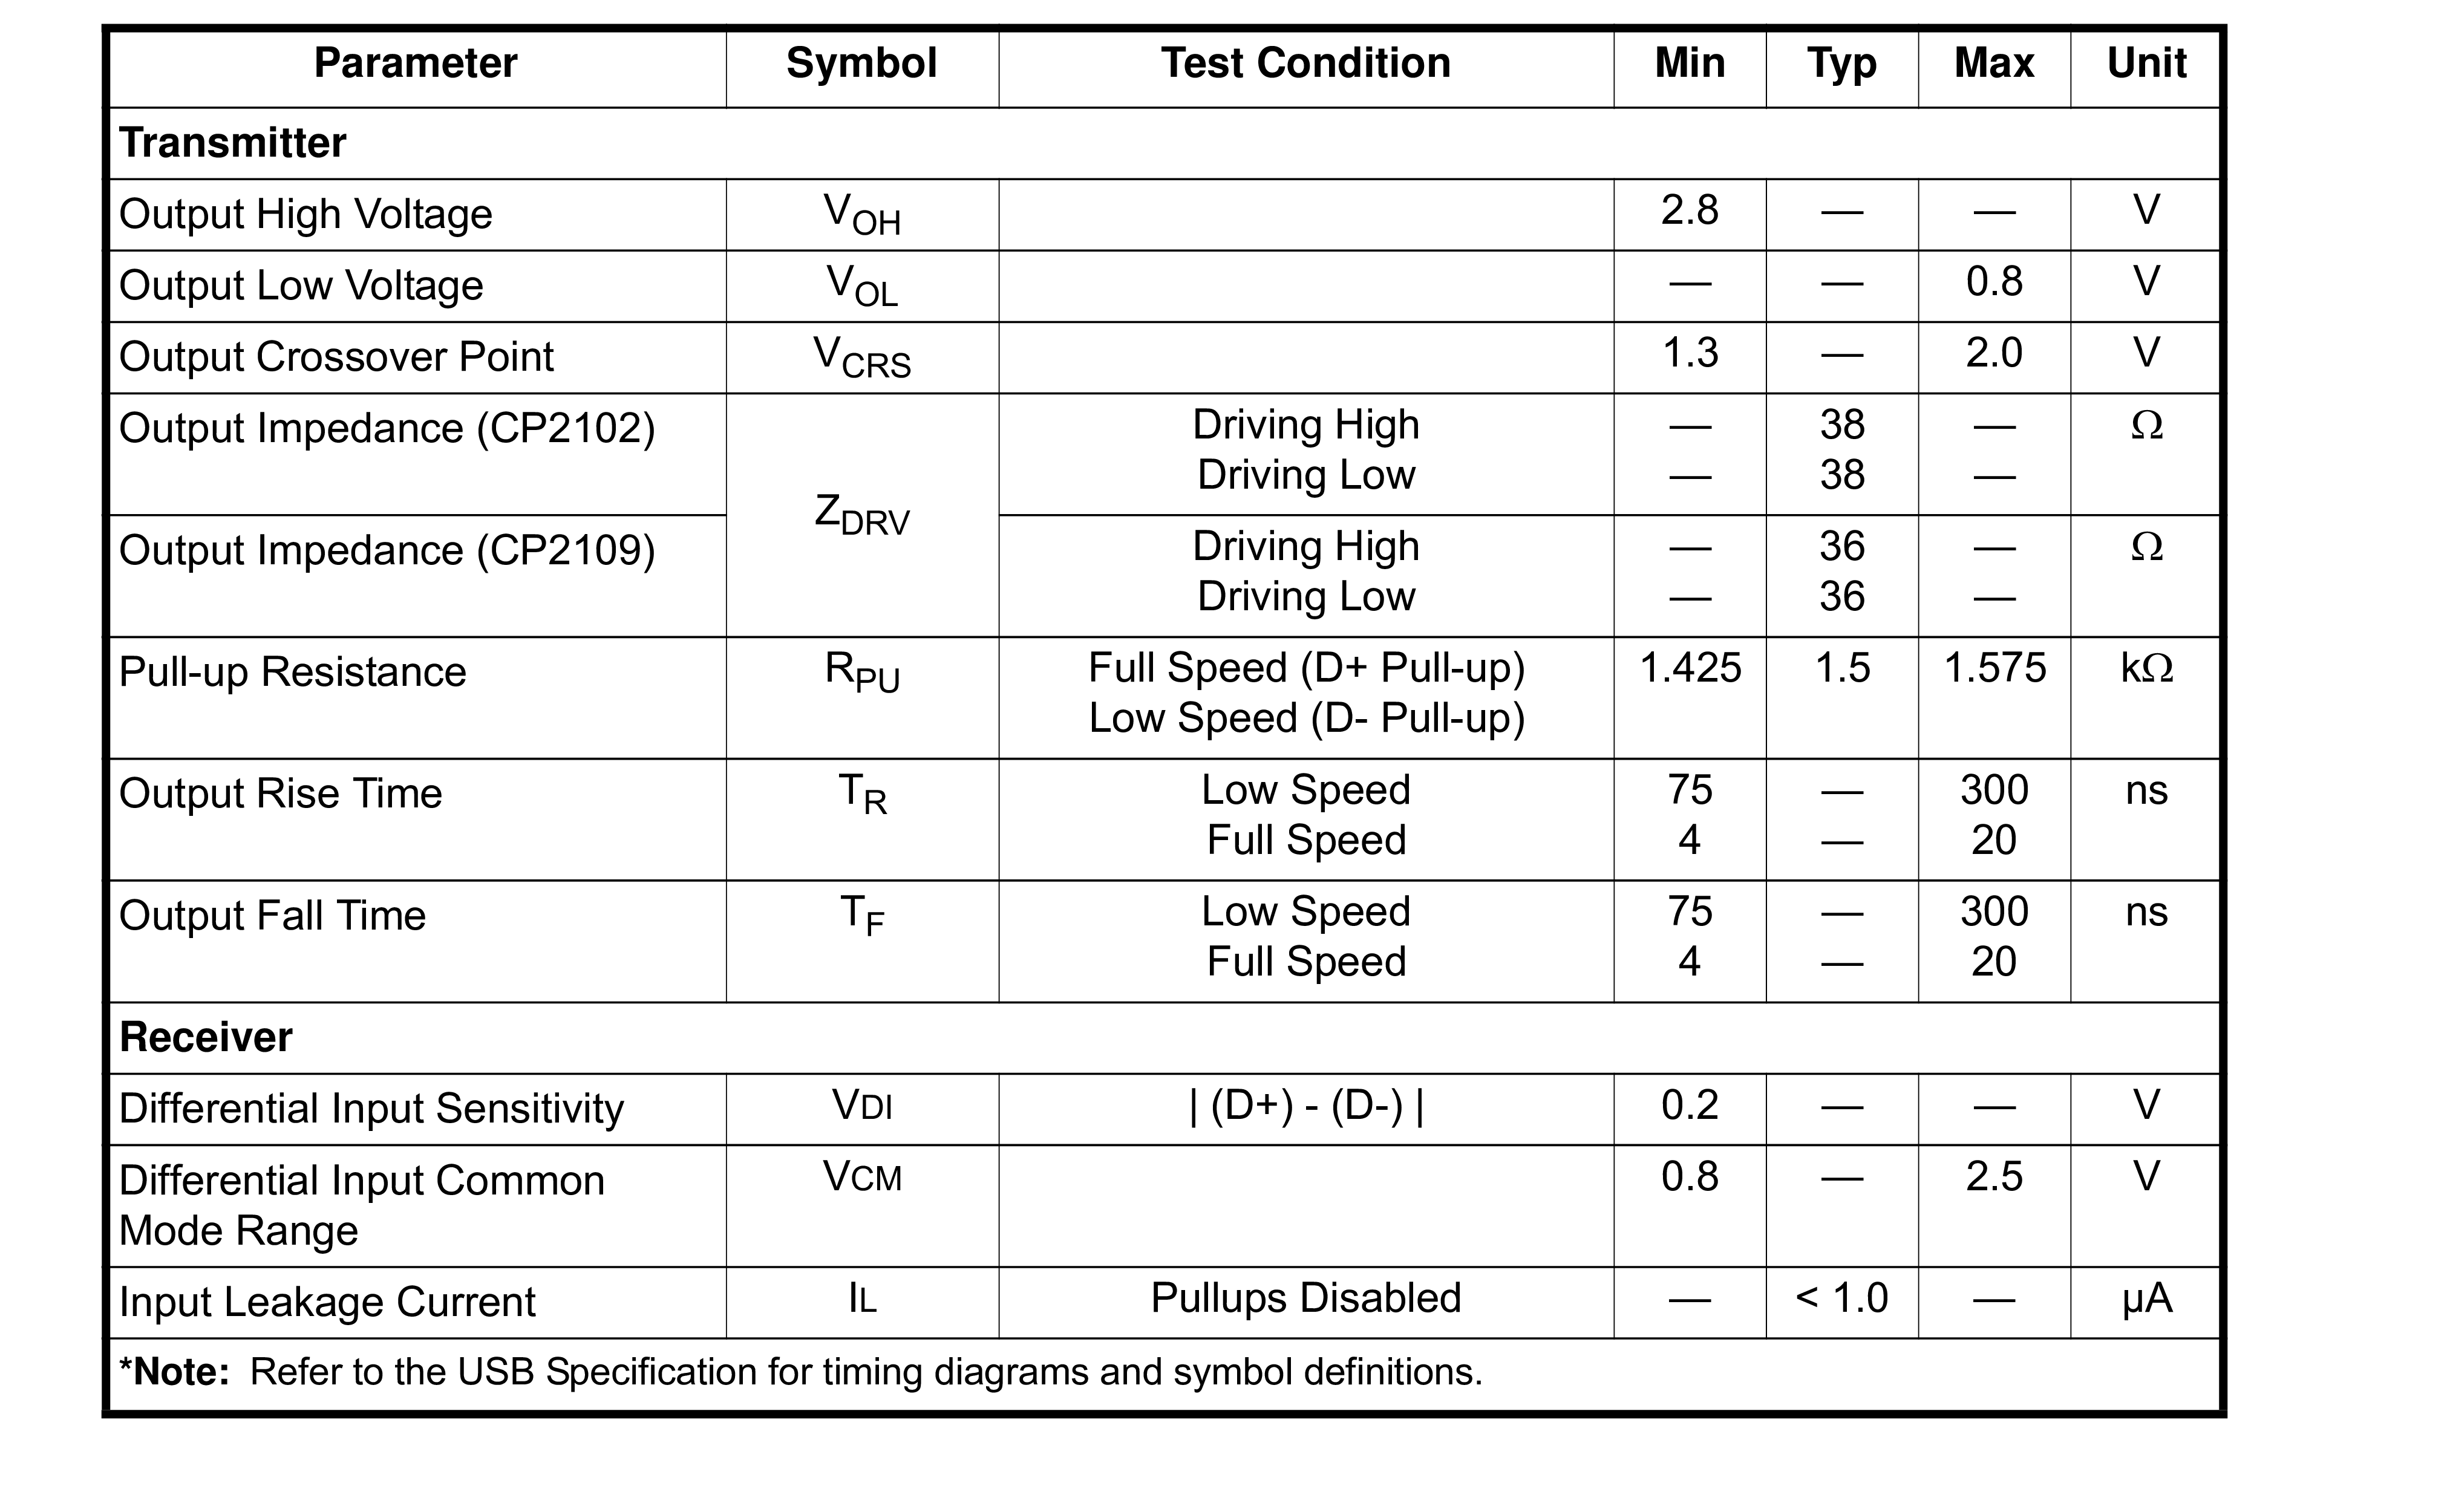
\includegraphics[width=\textwidth]{./img/usartvolt.png}
  \caption{USART Transceiver Electrical Specifications}\label{iso7816usartspecific}
\end{figure}

STM32在端口配置上具有比较强的灵活性,可以按照需要将部分端口配置到不同管脚。这里我们不
使用重定位功能,因此管脚配置为默认配置。此外,为了方便监测串口收发情况以及系统运行情况
,这里使用三只LED二极管,分别表示系统有Tx、Rx活动,以及系统的心跳信号。

最终管脚部署如下表\ref{iotable}所示。

\begin{table}[h]
\centering
\caption{IO Allocation Table}
\label{iotable}
\begin{tabular}{|c|c|c|c|c|}
\hline
端口用途 & 端口组别 & 端口号 & 端口工作模式 & 端口工作频率 \\\hline
串口Tx   & GPIO\_A  & 9     & AF\_PP    & 50MHz \\
串口Rx   & GPIO\_A  & 10   & IN\_FLOATING  & 50MHz \\
Tx指示   & GPIO\_E  & 7   & AF\_PP  & 50MHz \\
Rx指示   & GPIO\_E  & 8   & AF\_PP  & 50MHz \\
心跳指示   & GPIO\_E  & 9   & AF\_PP  & 50MHz \\
\hline\end{tabular}\end{table}

\subsection{片上的串口通信设备}

STM32为USART设备提供了两种片上通信模式。一种是传统的内存访问模式,另外一种是DMA模
式。通过使用DMA模式,结合桶状寄存器,STM32可以有效的提高USART访问速度。由于这种方
法涉及比较复杂的总线通信原理,这里略去不提,使用传统的内存访问模式完成串口通信设备
的操作。

\subsubsection{串口设备通信要素}

简单的讲,两线串口通信的原理就是,双方约定好相同的传输速度后,按照同一种解析方式,
对线路上的载波进行采样,并转化为数字信号的过程。这一传输速度就被称为“波特率”,其
单位为bps(比特每秒)。显然,要确保通信畅通,需要保证双方波特率一致,而波特率是通
过时钟分频得到的。也就是说,要保证:

\begin{enumerate}
\item 时钟准确
\item 时钟分频值准确
\end{enumerate}

工业上常用的波特率值,是150bps依次乘2之后得到的值,如300bps, 600bps, 1200bps……等。
比较常用的两个值是9600bps和115200bps。如果现场通信条件较差,波特率也要降低,以保证
信号传输完整。

串口通信是以帧的形式进行传输的,每个帧中要容纳固定个数的字节,否则双方匹配错误,
会产生通信问题。此外,在长距离通信中,为了尽量降低通信的错误率,串口通信引入了奇偶
校验位这个概念,对发送数据中的0或者1计数,以保证错误能及时被发现。另外,由于历史
原因,串口通信还支持基于硬件的流量控制机制。这些通信措施具体解释起来比较复杂,就不
再赘述了。

\subsubsection{波特率和时钟的对应关系}

按照时钟图,STM32的波特率和时钟之间有如下关系:
$$ Bandrate = f_{ck} / (16 * {USARTDIV}) $$
其中,$f_{ck}$是设备对应时钟总线的时钟频率,$USARTDIV$则为无符号浮点数,被分部存放在
\lstinline{USART_BRR}寄存器中。通信过程中,分频器会通过调取这个值,和系统时钟处理,
得到合适的分辨率。手工计算这个值比较麻烦,因此,在CMSIS子系统中,提供的
\lstinline{USART_init}函数,可以在处理结构体的过程中,计算这两个寄存器对应的初值。

需要注意的是,由于这个时钟直接受系统时钟的影响,因此在设置波特率的时候,也要考虑到总线
频率过高或过低对波特率的影响。比如,系统时钟为72MHz时,是无法得到600bps的波特率的。
这一点可以通过重设对应串口所在的总线时钟来解决。此外,由于这一机制本身存在一定漏
洞,分到的波特率不能总保证准确,如总线时钟为36MHz时,想得到115200bps的波特率,就
存在越$0.15\%$的误差。在部分程序中,这个误差是不能接受的。可以通过定时重启串口设备
及对应总线,来解决这个问题。关于误差计算的详细问题,请参考芯片设计手册第二十七章
第三节的相关内容,这里不再详述。

\subsubsection{通信设备事件处理}

通信主要分为发信和收信两个部分。由于CMSIS核系统已经提供了一定的框架,我们可以不用
手动对各个寄存器置位,但了解收发过程是很有必要的。为了叙述方便,我们假定通信中每个
字节为一个帧,每个数据包为一个字符串(也就是有多个帧)。

发送数据之前,程序需要对寄存器进行初始化,包括设定停止位、数据位,等等。之后启动串口,
这时串口进入初始化阶段,用户程序需要等待\lstinline{USART_SR->TXE}被置位,这意味着串
口已经准备好,可以发送数据。这时才能向\lstinline{USART_DR}的低八位中写入数据,写入后
,\lstinline{TXE}位会被自动清零,程序需要再次等待其被硬件置位,之后可以继续发送数据
,进行循环。最后一组数据发送完后,如果需要关闭串口,要等待\lstinline{TC}置位,防止
数据丢失。如果对程序的实时性有要求,可以不在此处等待,而采用中断方式,防止时间片抢占
。

接受数据时一般采用中断方式,减少CPU占用。中断服务子程序判断中断来源后,按照需要会读取
\lstinline{USART->DR}中的数据,此时这里的数据是接受到的字节码。读寄存器的同时,
\lstinline{RXNE}会自动清空,表示此时移位寄存器可用。这时,USART设备会把有可能到来的下
一个字节送入移位寄存器中,再次置位\lstinline{RXNE},表示又有了新的数据可以处理,同时
触发中断。如果此时还在处理之前的数据,则会产生一个咬尾中断,按照标准方法处理。若在此
期间再次产生一个中断,那么数据将会丢失。因此,在接受数据时,一定要保证速度尽量快,在
波特率比较高的时候更为重要,有必要的话可以使用多缓冲区或DMA方式。

\subsection{简单程序开发技巧}

现场调试过程中,偶尔会碰到一些特殊情况,比如没有JTAG接口可以引出,或者程序无法在线调
试。这种时候,除了利用dump分析方法以外,还可以使用其他方法排查故障。

一种比较常用的方法就是借助可用的IO口接入外接设备,借助IO口电平排查。比如这次,程序中
借助一个定时器和一个IO口,每隔一段时间闪动一次LED,表示CPU工作正常。但某个版本的代码
中,一旦发送特定数据,LED灯就不再闪动。这时就可以推测,在数据发送过程中,可能出现了死
循环或者一些内存错误。通过排查,确定有一个循环条件书写不正确,导致中断服务子程序陷入
循环,无法处理其他请求。

另外就是,善用编译器的预编译指令,能在保证程序结构完整的情况下,简化程序大小。这对于
嵌入式程序开发很有好处。比如,在调试退格功能的过程中,需要得知退格键对应的键码。在没
有调试器的情况下,可以让下位机把键码转化为字符串输出到上位机。但这个功能在调试时候是
不需要的,因此就可以使用如下清单\ref{defines}的预编译指令:
\begin{lstlisting}[caption={Usage of pre-defined commands},label={defines}]
#ifdef DEBUG
//Debug code
#else
//Normalcode
#endif
\end{lstlisting}
这样,在需要使用调试代码的时候,只要加入一行\lstinline{#define DEBUG}即可,在生产版
本中,则可用\lstinline{#undef DEBUG}或直接清除上述宏定义,即可完成代码屏蔽工作。

\section{程序运行和分析}

程序主文件如清单\ref{mainc}所示,这里对代码分片进行大致讲解。

在35行之前,是对有关函数和宏的定义。这里把LED灯和USART设备对应IO口都做了重定向处理,
提高代码可读性;此外,宏定义\lstinline{blink}用于切换LED灯状态,另两个宏则用于处理
串口的发送数据。从\lstinline{USART1_SENDOUT}的代码中,就可以看到,在发数据之前,要
等待一段时间,直到标志被置位后才可继续发送。

主函数完成初始化之后,向串口输出一条信息,表示启动完成,可以接受输入,之后进入死循环
,不完成实际工作。GPIO的初始化过程和前几次实验大同小异,主要注意的是在配置端口的过程
中,要关注IO口的工作模式是否和期望值相符。USART的初始化过程依旧利用CMSIS中的结构体完
成,注意这里我对每个值都做了初始化,这是为了明确部分值的作用,生产环境中部分值可以不
填。此外,\lstinline{USART_Mode}这一项是两个值的’或‘,意味着两个功能同时发挥作用,
这也是大多数情况下串口的标准配置。最重要的是,由于波特率设定为600bps,在系统的主配置
文件中,最好把系统时钟调整为24MHz,防止出现问题。

本次实验只有USART和心跳灯涉及到中断,这里的中断都用\lstinline{NVIC_EnableIRQ}函数进
行开启。在没有其他特殊要求的情况下,这种开启方法比较便捷。此外,需要注意的是,在NVIC
中开启中断之前,务必先设定对应片上设备的中断使能,并清理必要的标志位,以免造成不可预
料的问题。

125行开始的就是串口数据处理函数,这里的处理流程很简单,因此没有另开函数,而直接在服务
体内完成操作。除了退格和回车需要特殊处理之外,其他的数据原样发送即可。这里就采用了之前
说的调试技巧,利用预编译指令屏蔽掉了部分代码。

代码分析就到这里了,下面是对程序的演示过程,图\ref{pgload},\ref{pgsend},
\ref{pgedit}分别演示了程序启动、发送数据,以及删除和换行操作的效果图。

\begin{figure}[h]
  \centering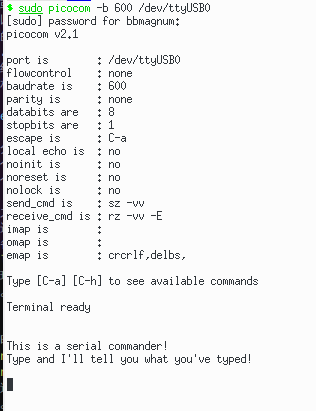
\includegraphics{./img/pgload.png}
  \caption{USART Teletyper has loaded}\label{pgload}
\end{figure}
\begin{figure}[h]
  \centering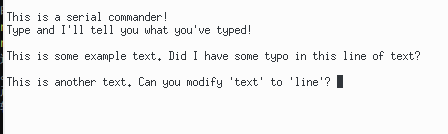
\includegraphics{./img/pgsend.png}
  \caption{Send some text to USART Teletyper (with a few wrong text)}\label{pgsend}
\end{figure}
\begin{figure}[h]
  \centering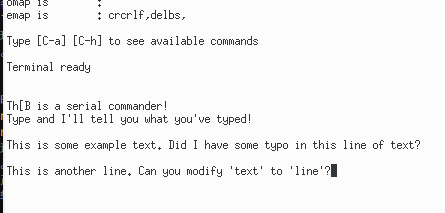
\includegraphics{./img/pgedit.png}
  \caption{Use backspace to modify wrong words}\label{pgedit}
\end{figure}


\section{程序代码}

\begin{lstlisting}[caption={Main file},label={mainc}]
#include "stm32f10x.h"

#define blink(group, pin)   do{if (GPIO_ReadOutputDataBit((group), (pin))) \
  GPIO_ResetBits((group), (pin)); \
  else GPIO_SetBits((group), (pin));}\
  while(0);
  
void GpioInitalize(void);
void UsartInitalize(void);
void TimerInitalize(void);

#define UsartTxPort GPIO_Pin_9
#define UsartRxPort GPIO_Pin_10
#define UsartGroup GPIOA
#define UsartGPIOClock RCC_APB2Periph_GPIOA
#define UsartClock RCC_APB2Periph_USART1

#define LEDTxPort GPIO_Pin_7
#define LEDRxPort GPIO_Pin_8
#define LEDRunPort GPIO_Pin_9
#define LEDGroup GPIOE
#define LEDGPIOClock RCC_APB2Periph_GPIOE

#define USART1_SENDOUT(data) do{USART_SendData(USART1,data);\
  blink(LEDGroup, LEDTxPort);\
  while(USART_GetFlagStatus(USART1, USART_FLAG_TC) == RESET);}while(0);
#define USART1_SENDCRLF() do{          USART_SendData(USART1,'\r');\
  while(USART_GetFlagStatus(USART1, USART_FLAG_TC) == RESET);\
  USART_SendData(USART1,'\n');}while(0);
#define ISDBG
#undef ISDBG

void printstr(char* str);

int main(void){
  //Initalize On-chip Periphals
  GpioInitalize();
  UsartInitalize();
  TimerInitalize();
  
  printstr("\n\n");
  printstr("This is a serial commander!\n");
  printstr("Type and I'll tell you what you've typed!\n");
  while(1);
}


void GpioInitalize(void){

  GPIO_InitTypeDef gpio_initval;

  /* Open clock */
  RCC_APB2PeriphClockCmd(LEDGPIOClock, ENABLE);
  RCC_APB2PeriphClockCmd(UsartGPIOClock, ENABLE);

  gpio_initval.GPIO_Speed = GPIO_Speed_50MHz;
  /* Tx port set*/
  gpio_initval.GPIO_Pin = UsartTxPort;
  gpio_initval.GPIO_Mode = GPIO_Mode_AF_PP;  //Need stronger output
  GPIO_Init(UsartGroup, &gpio_initval);
  /* Rx port set*/
  gpio_initval.GPIO_Pin = UsartRxPort;
  gpio_initval.GPIO_Mode = GPIO_Mode_IN_FLOATING;  //Need weeker input
  GPIO_Init(UsartGroup, &gpio_initval);

  /* LEDs Set*/
  gpio_initval.GPIO_Pin = LEDTxPort;  //Tx led
  gpio_initval.GPIO_Mode = GPIO_Mode_Out_PP;
  GPIO_Init(LEDGroup, &gpio_initval);
  gpio_initval.GPIO_Pin = LEDRxPort;  //Rx led
  gpio_initval.GPIO_Mode = GPIO_Mode_Out_PP;
  GPIO_Init(LEDGroup, &gpio_initval);
  gpio_initval.GPIO_Pin = LEDRunPort;  //heartbeat led
  gpio_initval.GPIO_Mode = GPIO_Mode_Out_PP;
  GPIO_Init(LEDGroup, &gpio_initval);

}


void UsartInitalize(void){

  USART_InitTypeDef usart_initval;
  
  /* Clock Initalize*/
  RCC_APB2PeriphClockCmd(UsartClock, ENABLE);    
  /* Configurements of USART1 */
  usart_initval.USART_BaudRate = 600;    //baudrate is 600. notice sysclock
  usart_initval.USART_HardwareFlowControl 
    = USART_HardwareFlowControl_None ;  //no flow control
  usart_initval.USART_StopBits = USART_StopBits_1;//1s
  usart_initval.USART_WordLength = USART_WordLength_8b;  //8d
  usart_initval.USART_Parity = USART_Parity_No;    //No check
  usart_initval.USART_Mode = 
    USART_Mode_Rx | USART_Mode_Tx;  //Do both job
  /* Write configure */
  USART_Init(USART1, &usart_initval);
  /* USART1 IRQn Triggerable */
  USART_ITConfig(USART1, USART_IT_RXNE, ENABLE);
  /* USART1 Bootup */
  USART_Cmd(USART1, ENABLE);
  /* USART1 IRQn NVIC Interruptable */
  NVIC_EnableIRQ(USART1_IRQn);
}

void TimerInitalize(void){

  TIM_TimeBaseInitTypeDef tim_tb_initval;

  //Enable timer of heart beat
  RCC_APB1PeriphClockCmd(RCC_APB1Periph_TIM2, ENABLE);  
  TIM_DeInit(TIM2);   //Reset to default
  /* Set timer to 4Hz */
  tim_tb_initval.TIM_Prescaler = 36000; 
  tim_tb_initval.TIM_ClockDivision = TIM_CKD_DIV1;  
  tim_tb_initval.TIM_CounterMode = TIM_CounterMode_Up;  
  tim_tb_initval.TIM_Period =  500-1;      
  TIM_TimeBaseInit(TIM2, &tim_tb_initval);  //apply settings
  TIM_ClearFlag(TIM2, TIM_FLAG_Update);    //clear flag
  TIM_ITConfig(TIM2, TIM_IT_Update, ENABLE);  //can set interruption
  TIM_Cmd(TIM2, ENABLE);    //enable Timer2
  NVIC_EnableIRQ(TIM2_IRQn);  //Enable IRQ in NVIC

}

void USART1_IRQHandler(void){
  unsigned char x;
  if (USART_GetITStatus(USART1, USART_IT_RXNE)==SET){
    /* Received a byte */
    blink(LEDGroup, LEDRxPort);
    x=USART_ReceiveData(USART1);  //RXNE will be hw-cls by reading data
    while(USART_GetFlagStatus(USART1, USART_FLAG_TC) == RESET);  //wait till idle
    if (USART_GetITStatus(USART1, USART_IT_TXE)==RESET)  //make sure sendable
    switch (x) {
      case '\r'://make special process for CRLF
        USART1_SENDCRLF();
        break;
      case 0x7F:
      USART1_SENDOUT(8);
      USART1_SENDOUT(' ');
      USART1_SENDOUT(8);
        break;
      default:
      #ifdef ISDBG
        USART1_SENDOUT('*');
        USART1_SENDOUT(x);
        USART1_SENDOUT('=');
        USART_SendData(USART1, x);//send data back
        x=(x>>4)|(x<<4);
        USART1_SENDOUT((x&0xf)>10?(x&0xf)-10+'A':(x&0xf)+'0');//send data back
        x>>=4;
        USART1_SENDOUT((x&0xf)>10?(x&0xf)-10+'A':(x&0xf)+'0');//send data back
        USART1_SENDOUT('*');
      #else
        USART1_SENDOUT(x);
      #endif
    }
  }
}

void TIM2_IRQHandler(void){
  if (TIM_GetITStatus(TIM2, TIM_IT_Update)!=RESET){
    TIM_ClearITPendingBit(TIM2, TIM_FLAG_Update);  //Clear IT Flag
    blink(LEDGroup, LEDRunPort);  //Show the heartbeat
  }
}

void printstr(char* str){
  while(*str!='\0'){
    if (*str == '\n')
      USART1_SENDOUT('\r');
    USART1_SENDOUT(*str++);
  }
}
\end{lstlisting}
\end{document}
